\section{Ergo's Native Token}

\subsection{Currency And Emission}
\label{sec:currency}

The native currency of \Ergo{} platform is \Erg{} token, which unique property is
that it is the only currency to pay for storage rent in \Ergo{}~(see Section~\ref{sec:survivability} for more details).
One \Erg{} token is divisible to up to $10^9$ smallest units, \nanoErg{}s.

All \Erg{} tokens that will ever circulate in the system are presented in
the initial state and are divided into 3 parts~(boxes):

\knote{no any notion of a box was introduced before, the introduction is sudden}
\dnote{I propose to add section about Ergo state before this one and introduce box notion in it}

\begin{itemize}
    \item{\em No premine proof.} This box contains exactly one~\Erg{} and is protected by the script
    that is preventing it from spending by anyone.
    Thus, it is a long-lived box that will stay in the system until storage-rent component
    destroys it.
    Its main purpose is to prove that \Ergo{} mining was not started privately by anyone before
    the declared launch date.
    To achieve this, additional registers of this box contains latest titles from media (The Guardian, Vedomosti, Xinhua)
    as well as latest block identifiers from Bitcoin and Ethereum.
    Thus, \Ergo{} mining could not be started before certain events in the real world and the
    cryptocurrency space.

    \item{\em Treasury.} This box contain 4,330,791.5 \Erg{} that will be used to fund \Ergo{}
    development.
    Its protecting script~\cite{link to corresponding ergo tree} consists of two parts.

    First, it ensures that only a predefined portion of the box value is unlocked.
    During blocks 1-525,599 (2 years) 7.5 \Erg{} will be released every block,
    during blocks 525,600-590,399 (3 months) 4.5 \Erg{} will be released every block, and finally,
    during blocks 590,400-655,199 (3 months) 1.5 \Erg{} will be released every block.
    This rule ensures the presence of funds for \Ergo{} development for at least 2.5 years and, at any moment of time,
    rewards do not exceed 10\% of the total number of coins in circulation.

    Second, it has custom protection from unexpected spending.
    Initially, it requires that spending transaction should be signed by at least 2 of 3 secret keys
    that are under control of initial team members. When they spend the box, they are free to
    change this part of the script as they wish, for example by adding new members to protect foundation
    funds, or switching to threshold by special token ownership~\cite{link to ...}.

    During the first year, these funds are going to be used to cover pre-issued EFYT token~\cite{our website},
    after that, they will be distributed in a decentralized manner via community voting.


    \item{\em Miners reward.} This box contains 93,409,132 \Erg{} that will be collected by block miners
    as rewards for their work.
    Its protecting script~\cite{link to corresponding ergo tree} requires that spending transaction
    should have exactly two outputs with the following properties:

    \begin{itemize}
    \item{} the first output should be protected by the same script and number of \Erg{} in it should
    equal to the remaining miners' reward.
    During blocks 1 - 525,599 (2 years) miner will be able to collect 67.5 \Erg{} from this box,
    during blocks 525,600 - 590,399 (3 month) miner will be able to collect 66 \Erg{} and after
    that block reward will be reduced by 3 \Erg{} every 64,800 blocks (3 months) until it reaches zero
    at block 2,080,799.

    \item{} the second output should contain the remaining coins and should be protected by the following condition:
    it can be spent by a miner that solved the block's PoW puzzle and not earlier than 720 blocks after the current block.
    % These restrictions are done to prevent mining pools formation, see~\ref{sec:autolykos} for more details.
    \end{itemize}

\end{itemize}

All these rules results in the following curve of the number of coins in circulation with time:

\begin{figure}[H]
    \centering
    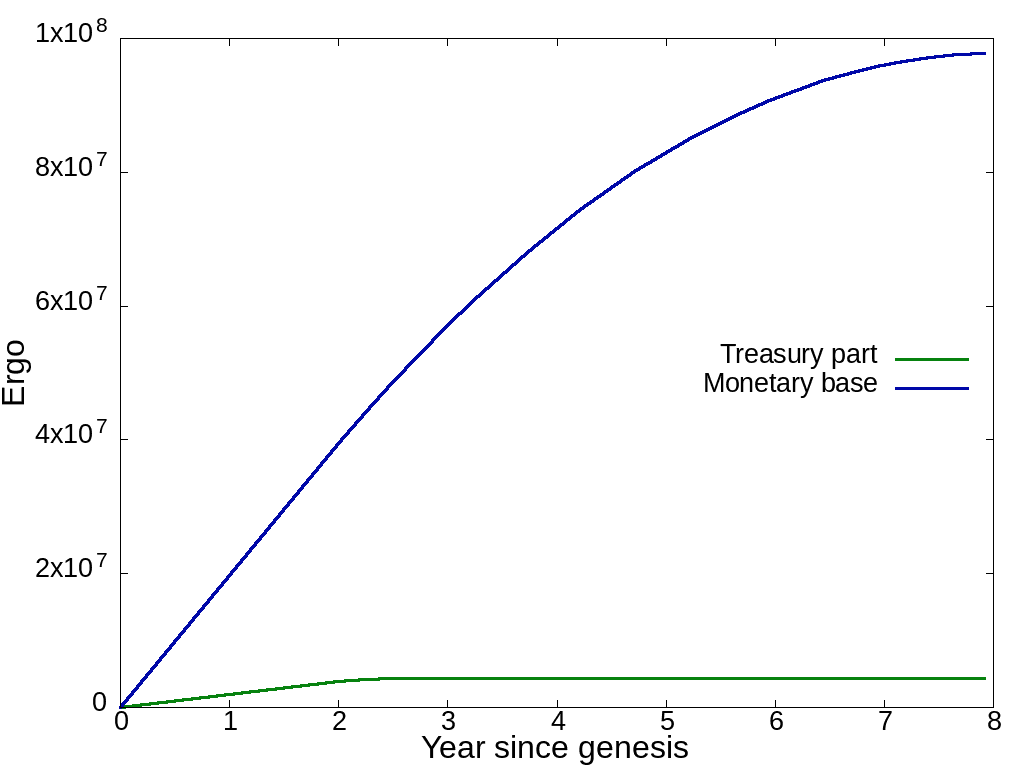
\includegraphics[width=\textwidth]{img/emission.png}
    \caption{Ergo emission curve
    \label{fig:emission} }
\end{figure}


\subsection{Ergo's Token Value}
 \label{sec:ergo-value}

 \dnote{I think it might be correct to rename previous section "Currency And Emission"~\ref{sec:currency} to
 "Ergo native token" and include this subsection into it}

 \dnote{Bitcoin have utility usage to pay for network resources as well as Ethereum has a utility usage to pay for
 computations~(we've also discussed it in "Systematic approach to cryptocurrency fees" paper). Also Ethereum emission
 rate was only reduced making it better and better as a store of value and is following "set in stone social contract" that
 it will reach zero when it will switch to PoS. Keeping in mind lost coins, Ethereum may be better then Ergo even
 right now, as far as efficient number of coins in circullation may reduce with time unlike Ergo.}

 \dnote{Instead of comparision of medium of exchange or store of value properties with BTC/ETH, I propose to
 describe, that Erg is utility token with the different purpose~(pay storage fee) and also have limited
 supply~(that would be natural if we'll move this part into previous section)}


 In this section, we are going to provide some reflections on the nature of the native Ergo token. For starters, we note that
 any currency is about three main functions: a medium of exchange, a unit of account, and a store of value.

 Bitcoin, being historically the first digital scarce asset, is perfect as store-of-value. It is even better than
 gold under certain assumptions~(such as SHA-256 hash function not being broken, and majority of miners are not willing
 to destroy the Bitcoin), as emission is limited and known in advance. However, being perfect store-of-value also means
 to be not so good as medium-of-exchange. In particular, if one knows that Bitcoin is indeed the best tool to store
 value in the long term, he would use fiat whenever possible in order to collect more bitcoins.

 On the other hand, Ethereum is not just a currency, but a utility token used to pay for computations over the
 "decentralized world computer" (or "fully replicated programmable calculator"). However, Ethereum is not good as
 store-of-value, as emission in endless, and, historically, can be changed easily by the community core along with
 critical system assumptions.

 Ergo combines best from these two top blockchains. Emission is predefined and limited, more, it will be finished within
 just ten years. The system assumptions are set in stone with precisely defined {\em social contract}~\ref{sec:social}. Also,
 Ergo is a utility token used to pay for storage rent. This storage rent is making the system more stable. Last, Ergo is
 suitable to build monetary systems on top of it with properties different from Ergo native token itself. However,
 participating in such systems would require to use Ergo native token as well in order to pay storage rent.
